\documentclass{article}
\usepackage[utf8]{inputenc} % Codificación de caracteres
\usepackage{graphicx}
\usepackage{listings}
\graphicspath{ {images/} }

\title{Tipos de Datos mutables e inmutables}
\author{Valery Triana}
\date{\today} % Fecha actual


\begin{document}
\maketitle

\section{Java}

\subsection{Introducción}
A continuación se presentan los tipos de datos primitivos en Java y sus características.

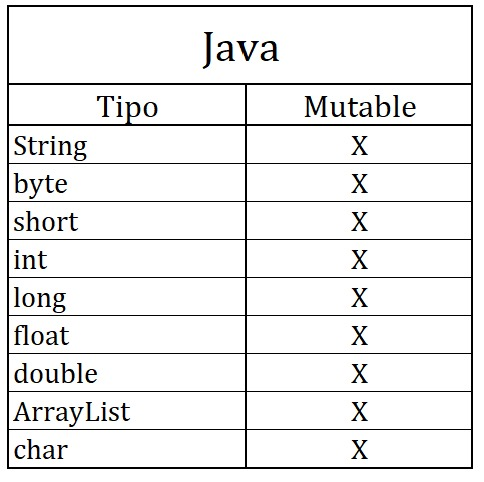
\includegraphics[width=0.5\textwidth]{javaTabla.jpg} % Ajusta el ancho según sea necesario

\subsection{Codigo de ejemplo}
\begin{lstlisting}[language=Java, caption=Ejemplo de código en Java]
import java.util.ArrayList;

public class MutableExample {
    public static void main(String[] args) {
        // Creamos un ArrayList mutable de cadenas
        ArrayList<String> mutableList = new ArrayList<>();
        
        // Añadimos elementos al ArrayList
        mutableList.add("Hola");
        mutableList.add("Mundo");
        mutableList.add("!");

        // Modificamos el primer elemento
        mutableList.set(0, "Saludos");

        // Eliminamos el segundo elemento
        mutableList.remove(1);

        // Imprimimos el ArrayList modificado
        System.out.println("ArrayList mutable modificado: " + mutableList);
    }
}


\end{lstlisting}

En este ejemplo, la complejidad temporal es O(n), donde n es la cantidad de elementos de la lista. Esta complejidad se debe al método remove, el cual, al retirar un elemento de la lista, debe reacomodar los que quedan.


\section{Golang}
\subsection{Introducción}
A continuación se presentan los tipos de datos primitivos en Golang y sus características.

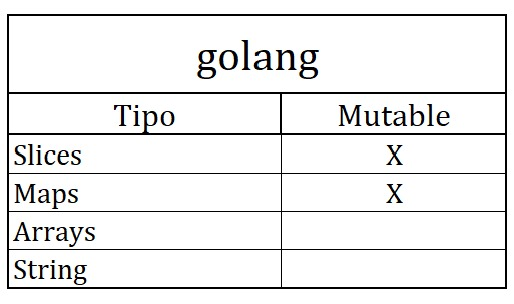
\includegraphics[width=0.5\textwidth]{golangTabla.jpg}

\subsection{Codigo de ejemplo}
\begin{lstlisting}[language=Golang, caption=Ejemplo de código en Golang]
package main

import "fmt"

func main() {
    // Creamos un slice mutable
    mutableSlice := []int{1, 2, 3}
    
    // Modificamos el slice
    mutableSlice[0] = 10
    mutableSlice = append(mutableSlice, 4)
    
    fmt.Println("Slice mutable modificado:", mutableSlice)
}
\end{lstlisting}

En este ejemplo, la complejidad temporal es O(1). Esto se debe a que crear un slice, modificar una posición específica y añadir un elemento al final del slice requieren un tiempo constante.

\section{Python}
\subsection{Introducción}
A continuación se presentan los tipos de datos primitivos en Python y sus características.

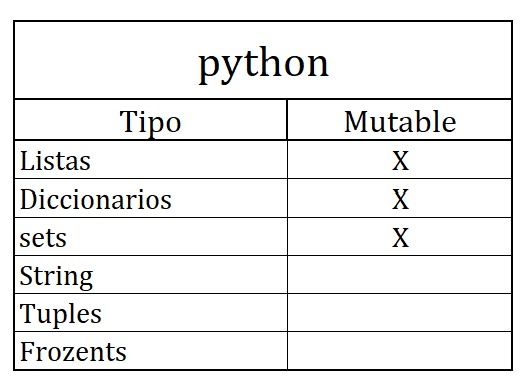
\includegraphics[width=0.5\textwidth]{pythonTabla.jpg}

\subsection{Codigo de ejemplo}
\begin{lstlisting}[language=Python, caption=Ejemplo de código en Python]
# Creamos una lista mutable
mutable_list = [1, 2, 3]

# Modificamos la lista
mutable_list[0] = 10
mutable_list.append(4)
\end{lstlisting}

En este ejemplo, la complejidad temporal es O(1), ya que tanto la creación de una lista, la modificación de un elemento en una posición dada y la adición de un elemento al final toman un tiempo constante.

\section{C++}
\subsection{Introducción}
A continuación se presentan los tipos de datos primitivos en C++ y sus características.

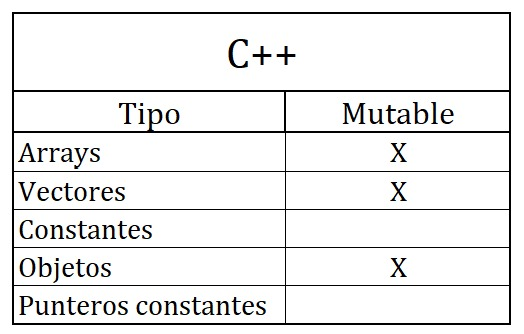
\includegraphics[width=0.5\textwidth]{c++Tabla.jpg}

\subsection{Codigo de ejemplo}
\begin{lstlisting}[language=C++, caption=Ejemplo de código en C++]
#include <vector>
#include <iostream>

int main() {
    std::vector<int> mutableVector = {1, 2, 3}; // Inicializamos un vector mutable
    mutableVector.push_back(4); // Agregar un nuevo elemento al final
    mutableVector[1] = 5; // Modificar el segundo elemento
    std::cout << "Vector mutable modificado:";
    for (int num : mutableVector) {
        std::cout << " " << num;
    }
    std::cout << std::endl;
    return 0;
}
\end{lstlisting}

En este ejemplo, la complejidad es O(n), donde n representa la cantidad de elementos en el vector. Aunque la creación de un vector, la adición de un elemento y la edición de un elemento en una posición dada toman un tiempo constante, el recorrido de cada elemento para imprimirlo implica una complejidad O(n), donde n es la cantidad de elementos.
\end{document}
